\section{Variedades Riemannianas}

\begin{definicao}
	Uma \emph{métrica Riemanniana} em uma variedade suave $M^n$ é uma correspondência $\langle , \rangle$ que associa a cada ponto $p \in M$, um produto interno $\langle , \rangle_p$ em $T_p M$ e que varia diferenciavelmente no sentido de que a função
	\begin{equation*}
		p \in M \mapsto \langle X(p), Y(p) \rangle_p
	\end{equation*}	
	seja diferenciável para qualquer $X,Y \in \mathfrak{X}(M)$.
\end{definicao}

\begin{definicao}
	Uma \emph{variedade Riemanniana} é um par $(M, \langle , \rangle)$.
\end{definicao}

\begin{observacao}
	Dado uma carta local $(U, \varphi)$ em $M$ com $\varphi \sim (x_1, \ldots, x_n)$. Denote por
	\begin{equation*}
		dx_1, \ldots, dx_n
	\end{equation*}	
	as 1-formas duais aos campos coordenados $\frac{\partial}{\partial x_1}, \ldots, \frac{\partial}{\partial x_n}$, ou seja,
	\begin{equation*}
		dx_i (p): T_p M \rightarrow \mathbb{R}
	\end{equation*}	
	é o funcional linear dado por
	\begin{equation*}
		dx_i (p) \frac{\partial}{\partial x_j} = \delta_{ij}
	\end{equation*}	
	onde $\delta_{ij} = 1$ quando $i=j$ e $\delta_{ij} = 0$ quando $i \neq j$. 
	
	Dados $p \in U$ e $v,w \in T_p M$, escrevamos
	\begin{align*}
		v &= \sum_{i=1}^n v_i \frac{\partial}{\partial x_i}(p) \text{ e }\\
		w &= \sum_{i=1}^n w_i \frac{\partial}{\partial x_i}(p)
	\end{align*}	
	Usando a bilinearidade da métrica obtemos
	\begin{align*}
		\langle v,w \rangle_p &= \left\langle \sum_{i=1}^n v_i \frac{\partial}{\partial x_i}(p), \sum_{i=1}^n w_i \frac{\partial}{\partial x_i}(p) \right\rangle_p\\
		&= \sum_{i,j = 1}^n v_i w_j \left\langle \frac{\partial}{\partial x_i}(p), \frac{\partial}{\partial x_j}(p) \right\rangle_p\\
		&= \sum_{i,j=1}^n v_i w_j g_{ij}(p)
	\end{align*}	
	onde $g_{ij}(p) = \left\langle \frac{\partial}{\partial x_i}(p), \frac{\partial}{\partial x_j}(p) \right\rangle_p$.
	
	Como $g_{ij} = g_{ji}$ e
	\begin{align*}
		dx_i (p) v &= dx_i (p) \left( \sum_{j=1}^n v_j \frac{\partial}{\partial x_j}(p) \right)\\
		&= v_i
	\end{align*}	
	e
	\begin{equation*}
		dx_i (p) w = w_i
	\end{equation*}	
	podemos escrever
	\begin{align*}
		\langle , \rangle &= \sum_{i,j=1}^n g_{ij} dx_i \otimes dx_j\\
		&= \sum_{i \leq j, i=1}^n \tilde{g}_{ij} dx_i dx_j
	\end{align*}	
	onde $\tilde{g}_{ii} = g_{ii} $ e $\tilde{g}_{ij} = 2g_{ij}$ se $i \neq j$.
\end{observacao}

\begin{exemplo}
	Em $\mathbb{R}^n$, identificamos
	\begin{equation*}
		\frac{\partial}{\partial x_i} (p) = e_i
	\end{equation*}	
	com $1 \leq i \leq n$ para qualquer $p \in \mathbb{R}^n$. Assim, a métrica $\langle , \rangle$ em $\mathbb{R}^n$ é dada por
	\begin{align*}
		\left\langle \frac{\partial}{\partial x_i}(p), \frac{\partial}{\partial x_j}(p) \right\rangle_p &= \langle e_i, e_j \rangle_p\\
		&= \langle e_i, e_j \rangle\\
		&= \delta_{ij}
	\end{align*}	
	ou seja
	\begin{align*}
		\langle , \rangle &= dx_1 dx_1 + \ldots + dx_n dx_n \\
		&= dx_1^2 + \ldots + dx_n^2
	\end{align*}
\end{exemplo}


\begin{exemplo}
	A métrica euclideana em $\mathbb{R}^2$ é dada por
	\begin{equation*}
		\langle , \rangle = dx^2 + dy^2
	\end{equation*}	
	Passando para coordenadas polares
	\begin{align*}
		x &= r \cos \theta\\
		y &= r \sin \theta
	\end{align*}	
	obtemos
	\begin{align*}
		dx &= \cos \theta dr - r \sin \theta d\theta\\
		dy &= \sin \theta dr + r \cos \theta d\theta
	\end{align*}	
	Assim,
	\begin{align*}
		\langle , \rangle &= dx^2 + dy^2\\
		&= dr^2 + r^2 d\theta^2
	\end{align*}
\end{exemplo}

\begin{exemplo}
	Considere a superfície de rotação $M^2$ em $\mathbb{R}^3$ parametrizada por
	\begin{equation*}
		\varphi(s,\theta) = (a(s) \cos \theta, a(s) \sin \theta, b(s))
	\end{equation*}	
	onde $a,b$ são funções diferenciáveis definidas em um intervalo aberto de $\mathbb{R}$, com $a>0$ e $\gamma(s) = (a(s),0,b(s))$ é a curva geratriz de $M^2$, com $\| \gamma'(s) \|^2 = (a'(s))^2 + (b'(s))^2 = 1$.
	
	Considere $M^2$ munida da métrica riemanniana $\langle , \rangle$ induzida de $\mathbb{R}^3$, i.e., cada plano tangente $T_p M$ está munido do produto interno usual de $\mathbb{R}^3$. Tais planos sao gerados pelas derivadas parciais
	\begin{align*}
		\frac{\partial \varphi}{\partial s} &= \varphi_s = (a'(s) \cos \theta, a'(s) \sin \theta, b'(s))\\
		\frac{\partial \varphi}{\partial \theta} &= \varphi_{\theta} = (-a(s) \sin \theta, a(s) \cos \theta, 0)
	\end{align*}	
	Assim,
	\begin{align*}
		\langle , \rangle &= \langle \varphi_s, \varphi_s \rangle ds^2 + 2 \langle \varphi_s, \varphi_{\theta} \rangle ds d\theta + \langle \varphi_{\theta}, \varphi_{\theta} \rangle d\theta^2\\
		&= ds^2 + a(s)^2 d\theta^2
	\end{align*}
\end{exemplo}

\begin{exemplo}
	Seja $f: M \rightarrow N$ uma imersão, i.e., $f$ é uma aplicação diferenciável tal que
	\begin{equation*}
		df(p): T_p M \rightarrow T_{f(p)} N
	\end{equation*}	
	é injetiva para qualquer $p \in M$. Suponha que $N$ esteja munida de uma métrica Riemanniana $\langle , \rangle^N$. Podemos definir uma métrica $\langle , \rangle^M$ em $M$
	\begin{equation*}
		\langle v,w \rangle_p^M := \langle df(p) v, df(p) w \rangle_{f(p)}^N
	\end{equation*}	
	Neste caso, dizemos que $f$ é uma \emph{imersão isométrica}.
\end{exemplo}

\begin{teorema}[Nash]
	Toda variedade suave $M$ pode ser mergulhada em algum espaço euclideano $\mathbb{R}^n$, i.e., existe uma imersão $f: M \rightarrow \mathbb{R}^n$ tal que sobre a imagem, $f$ é um homeomorfismo.
\end{teorema}

\begin{corolario}
	Toda variedade suave $M$ pode ser munida de métrica Riemanniana.
\end{corolario}

\begin{demonstracao}
	contenidos...
\end{demonstracao}

\begin{definicao}
	Uma \emph{conexão afim} em uma variedade suave $M$ é uma aplicação
	\begin{align*}
		\nabla: \mathfrak{X}(M) \times \mathfrak{X}(M) & \rightarrow \mathfrak{X}(M)\\
		(X,Y) & \mapsto \nabla_X Y
	\end{align*}	
	que satisfaz:
	\begin{enumerate}
		\item $\nabla_X (Y+Z) = \nabla_X Y + \nabla_X Z$
		\item $\nabla_{fX+gY} Z = f \nabla_X Z + g \nabla_Y Z $
		\item $\nabla_X (fY) = f \nabla_X Y + X(f) Y$
	\end{enumerate}
para todo $X,Y,Z \in \mathfrak{X}(M)$ e $f,g \in C^{\infty}(M)$.
\end{definicao}

\begin{observacao}
	$X(f)(p) = df(p)X(p)$, i.e., $X: C^{\infty}(M) \rightarrow C^{\infty}(M)$.
\end{observacao}

\begin{proposicao}\label{boa_definicao_conexao}
	Dados $p \in M$ e $X,Y \in \mathfrak{X}(M)$ o valor $(\nabla_X Y)(p)$ depende somente de $X(p)$ e da restrição de Y ao longo de uma curva diferenciável $\gamma: (-\epsilon, \epsilon) \rightarrow M$ com $\gamma(0)=p$ e $\gamma'(0)=X(p)$.
\end{proposicao}

\begin{figure}
	\centering
	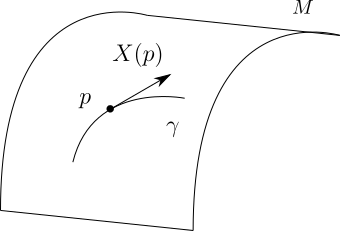
\includegraphics[scale=0.5]{images/curva_variedade.png}
	\caption{Descrição da proposição \ref{boa_definicao_conexao}}
\end{figure}

\begin{demonstracao}
	contenidos...
\end{demonstracao}

\begin{observacao}
	$ \Gamma_{ij}^k $ sao os símbolos de Christoffel de $ \nabla $ em relação a $ (U,\varphi) $.
\end{observacao}

\begin{observacao}
	$(\nabla_X Y)(p) = \nabla_{X(p)} Y$
\end{observacao}

\begin{teorema}\label{levi-civita}
	Dado uma variedade Riemanniana $(M,\langle , \rangle)$, existe uma única conexão afim $\nabla$ em $M$ chamada de \emph{conexão de Levi-Civita} de $M$ que satisfaz:
	\begin{enumerate}
		\item $X \langle Y,Z \rangle = \langle \nabla_X Y,Z \rangle + \langle Y, \nabla_X Z\rangle$
		\item $\nabla_X Y - \nabla_Y X = [X,Y]$
	\end{enumerate}
	onde $[X,Y]$ é o \emph{colchete de Lie} dado por
	\begin{equation*}
		[X,Y] = X(Y(f)) - Y(X(f))
	\end{equation*}
\end{teorema}

\begin{demonstracao}
	contenidos...
\end{demonstracao}

\begin{observacao}
	Dado um conexao $\nabla$ em $M$, satisfazendo a segunda propriedade do teorema \ref{levi-civita} e uma carta local $(U,\varphi)$ em $M$, com $\varphi \sim (x_1, \ldots, x_n)$, temos:
	\begin{equation*}
		\nabla_{\frac{\partial}{\partial x_i}} \frac{\partial}{\partial x_j} - \nabla_{\frac{\partial}{\partial x_j}} \frac{\partial}{\partial x_i} = \left[ \frac{\partial}{\partial x_i}, \frac{\partial}{\partial x_j} \right] =0
	\end{equation*}	
	mostrando que $\Gamma_{ij}^k = \Gamma_{ji}^k$, para todo $1 \leq i,j \leq n$
\end{observacao}

\begin{observacao}
	Seja $(U,\varphi)$ uma carta local de $M$ tal que $\varphi \sim (x_1, \ldots,x_n)$. Então
	\begin{equation*}
		\left[\frac{\partial}{\partial x_i},\frac{\partial}{\partial x_j}\right](f) = \frac{\partial}{\partial x_i} \left(\frac{\partial f}{\partial x_j}\right) - \frac{\partial}{\partial x_j} \left(\frac{\partial f}{\partial x_i}\right)
	\end{equation*}
\end{observacao}

\begin{observacao}
	A conexão de Levi-Cevita de $\mathbb{R}^n$ coincide com a derivada usual de campos vetoriais em $\mathbb{R}^n$.
	
	De fato, sejam $(x_1,\ldots,x_n)$ as coordenadas usuais de $\mathbb{R}^n$. Temos
	\begin{align*}
		\left\langle \frac{\partial}{\partial x_i},\frac{\partial}{\partial x_j}\right\rangle &= \delta_{ij}\\
		\left[\frac{\partial}{\partial x_i},\frac{\partial}{\partial x_j}\right] &= 0
	\end{align*}	
	Segue da formula de Koszul que
	\begin{equation*}
		\nabla_{\frac{\partial}{\partial x_i}} \frac{\partial}{\partial x_j} = 0, \forall 1 \leq i,j \leq n
	\end{equation*}	
	implicando que $\Gamma_{ij}^k = 0, \forall i,j,k$. 
	
	Dados $X,Y \in \mathfrak{X}(\mathbb{R}^n)$, escrevamos
	\begin{align*}
		X &= \sum_{i=1}^n a_i \frac{\partial}{\partial x_i} \text{ e }\\
		Y &= \sum_{j=1}^n b_j \frac{\partial}{\partial x_j}
	\end{align*}	
	onde $a_i,b_j \in C^{\infty}(\mathbb{R}^n)$. Usando a formula
	\begin{equation*}
		(\nabla_X Y)_{|U} = \sum_{k} \left(\sum_{i,j} a_i b_j \Gamma_{ij}^k + \sum_{i} a_i \frac{\partial b_k}{\partial x_i} \right) \frac{\partial}{\partial x_k}
	\end{equation*}	
	obtemos
	\begin{align*}
		\nabla_X Y &= \sum_{k} \left(\sum_{i} a_i \frac{\partial b_k}{\partial x_i} \right) \frac{\partial}{\partial x_k}\\
		&= \sum_{k} X(b_k) \frac{\partial}{\partial x_k}\\
		&= X(Y)
	\end{align*}
\end{observacao}

\begin{exemplo}
	Seja $\mathbb{R}_+^2 = \{(x,y) \in \mathbb{R}^2: y>0\}$ e $\langle,\rangle = \frac{1}{y^2} \left(dx^2+dy^2\right)$. Vamos calcular $\nabla_{\frac{\partial}{\partial x_1}} \frac{\partial}{\partial x_1}$, $\nabla_{\frac{\partial}{\partial x_2}} \frac{\partial}{\partial x_2}$ e $\nabla_{\frac{\partial}{\partial x_1}} \frac{\partial}{\partial x_2}$
\end{exemplo}

\begin{definicao}
	Uma imersão $f: M \rightarrow \tilde{M}$ entre variedades Riemannianas é dita de ser uma \textit{imersão isométrica} se
	\begin{equation}
	\label{imersao_isometrica}
	\langle X,Y \rangle = \langle f_* X, f_* Y \rangle,
	\end{equation}
	para quaisquer $p \in M$ e $X,Y \in T_p M$.
\end{definicao}

\begin{observacao}
	Se $f: M \rightarrow \tilde{M}$ é simplesmente uma imersão e $\langle , \rangle$ é uma métrica em $\tilde{M}$, a relação \eqref{imersao_isometrica} define uma métrica Riemanniana em $M$, chamada a \textit{métrica induzida} por $f$, em relação a qual $f$ torna-se uma imersão isométrica.
\end{observacao}

\begin{observacao}
	Dado uma imersão isométrica $f:M \rightarrow \tilde{M}$, denotaremos por $f^* T \tilde{M}$ o fibrado vetorial induzido sobre $M$, cuja fibra no ponto $p \in M$ é $T_{f(p)} \tilde{M}$. O complemento ortogonal de $f_* T_p M$ em $T_{f(p)} \tilde{M}$ é chamado o \textit{espaço normal} de $f$ em $p$, e será denotado por $T_p M^\perp$. O \textit{fibrado normal} $TM^\perp$ de $f$ é o sub-fibrado vectorial de $f^* T \tilde{M}$ cuja fibra em um ponto $p \in M$ é $T_p M^\perp$.
\end{observacao}

\begin{observacao}
	A conexão Levi-Civita $\tilde{\nabla}$ de $\tilde{M}$ induz uma única conexão $\nabla$ em $f^* T \tilde{M}$ de modo que
	\begin{equation*}
		\nabla_X (Z \circ f) = \tilde{\nabla}_{f_* X} Z
	\end{equation*}
	para quaisquer $p \in M$, $X \in \mathfrak{X}(M)$ e $Z \in \mathfrak{X}(\tilde{M})$. Identificaremos as conexões $\nabla$ e $\tilde{\nabla}$, e denotaremos a primeira também por $\tilde{\nabla}$. Dados $X,Y \in \mathfrak{X}(M)$, podemos decompor
	\begin{equation*}
		\tilde{\nabla}_X f_* Y = \left( \tilde{\nabla}_X f_* Y \right)^{\top} \oplus \left( \tilde{\nabla}_X f_* Y \right)^{\perp}
	\end{equation*}
	em relação à decomposição ortogonal
	\begin{equation*}
		f^* \tilde{M} = f_* TM \oplus TM^\perp
	\end{equation*}
\end{observacao}

\begin{proposicao}
	A aplicação
	\begin{equation*}
		\nabla_X Y = f_*^{-1} \left( \tilde{\nabla}_X f_* Y \right)^{\top}
	\end{equation*}
	define uma conexão simétrica e compatível com a métrica de $M$ e, portanto, coincide com a conexão de Levi-Civita de $M$.
\end{proposicao}

\begin{demonstracao}
	contenidos...
\end{demonstracao}

A aplicação $\alpha_f: \mathfrak{X}(M) \times \mathfrak{X}(M) \rightarrow \Gamma(TM^\perp)$ definida por
\begin{equation*}
	\alpha_f(X,Y) = \left( \tilde{\nabla}_X f_* Y \right)^\perp
\end{equation*}

é chamada a \emph{segunda forma fundamental} de $f$. Assim, podemos escrever a \emph{formula de Gauss} dada por
\begin{equation*}
	\tilde{\nabla}_X f_* Y = f_* \nabla_X Y + \alpha_f(X,Y).
\end{equation*}
Observe que, como
\begin{equation*}
	\tilde{\nabla}_X f_* Y - \tilde{\nabla}_Y f_* X = f_* [X,Y],
\end{equation*}
segue que $\alpha_f$ é simétrica. Alem disso, $\alpha_f$ é $C^{\infty}(M)$-linear, logo o valor de $\alpha_f(X,Y)$ num ponto $p \in M$ depende somente dos valores de $X$ e $Y$ em $p$.

O \emph{operador de forma} $A_{\xi}$ de $f$ num ponto $p \in M$ com relação a $\xi \in T_p M^\perp$ e definido pondo
\begin{equation*}
	\langle A_\xi X, Y \rangle = \langle \alpha_f(X,Y). \xi \rangle,
\end{equation*}
para quaisquer $X,Y \in \mathfrak{X}(M)$. Dados $X,Y \in \mathfrak{X}(M)$ e $\xi \in TM^\perp$, temos:
\begin{align*}
	\left\langle \tilde{\nabla}_\xi, f_* Y \right\rangle &= -\langle \xi, \tilde{\nabla}_X f_* Y \rangle\\
	&= - \langle \xi, \alpha_f(X,Y) \rangle\\
	&= - \langle A_\xi X, Y \rangle.
\end{align*}

Assim, a componente tangente de $\tilde{\nabla}_X \xi$ é $-f_* A_\xi X$. Por outro lado, a componente normal
\begin{equation*}
	\nabla_X^\perp = \left( \tilde{\nabla}_X \xi \right)^\perp
\end{equation*}
define uma conexão compatível em $TM^\perp$, chamada a \emph{conexão normal de} $f$. Isso nos dá a \emph{formula de Weingarten}:
\begin{equation*}
	\tilde{\nabla}_X \xi = - f_* A_\xi X + \nabla_X^\perp
\end{equation*}